We used the The ONE simulator~\cite{the-one} to simulate an opportunistic exchange of messages between nodes communicating over the BLE, using the empirical results from the testbed experiment to model the signal path loss with distance.
The simulation was repeated for 25 runs per configuration, using an Ubuntu 22.04 with a Intel(R) Xeon(R) Gold 6326 CPU @ 2.90GHz with 64 cores, and 247 GB of RAM. To run the simulations we used parallelization by spawning 60 parallel jobs. 
In each run, the nodes remain static and attempt to send the same amount of messages to all other nodes in the network, using an epidemic router to flood messages across the network.
The epidemic router is especially useful to simulate the scenario of message propagation in disaster zones, where it is critical to disseminate information as fast and as wide as possible.
In an epidemic routing scheme, every node sends all its messages to all of its neighbors, and each neighbor recursively repeats this iterative process until the final destination node for each message is reached.
In every simulator run, a host generates 20 messages to all other hosts in the network, with a size of 247 bytes each. A simulator run ends when all generated messages are either delivered or discarded. 

For the signal path loss model, we used the empirical data presented in table~\ref{tab:rssi-stats}, and interpolated for distances between the empirical measurements using the normal logarithmic path loss model laid out in equation 6 of \cite{pathloss}.
The path loss model is defined as follows:
$$
RSSI_d (dBm) = A - 10 * \alpha * \log_{10}(\frac{d}{d_0})
$$
where $RSSI_d$ is the received signal strength indicator at distance $d$ between source and destination nodes, $d_0$ is the distance at the nearest lower or equal reference point, $A$ is the RSSI at the nearest lower or equal reference distance $d_0$ (as measured by the testbed), $\alpha$ is the path loss exponent.
We wanted to evaluate the performance of the Bluetooth Low Energy running on 1M PHY mode, which means a symbol modulation rate of 1Mbps at $\le1$ meter.

A large 400$\times$400 meter L-shape building hall was generated, split to a grid of 12 equal-sized cells of 100 $\times$ 100 meters each assigned to a cluster consisting of six hosts, for a total of 72 hosts. Each host was randomly placed within the cluster cell assigned to it.
A random number generator that generates the node positions, whose seed is derived from the communication range, the message size, and optionally by the simulation run number, is used to ensure reproducibility of results.
The communication range is a configurable parameter which limits the radius of communication of the network interface that each node has: for simplification, a connection between two nodes can be established if they are within the communication radius of each other, and have direct line of sight.
A connection does not churn during a simulation run: once a connection is established it is maintained until the end of the simulation run.

\subsection{Model Insights}
Different topologies were generated by using the communication radii of [1,5,10,20,30,40,50,60,70,80,90,100] meters.
A simulation run configuration consists of a set of parameters, including the message generation rate, the maximum communication radius of each node, the maximum number of parallel connections (max node degree) each node can establish and maintain, and the communication mode: either exclusively intra-cluster communication to simulate clique-based short-range cluster communication, or inter-cluster communication to simulate long-range communication.
The same exact topology was repeated for [1,2,3,4,5,6,7,8,9,10,15,20] maximum node degrees, each for 25 runs, keeping the topologies invariant to the run number but changing them for each communication range, thereby shuffling the order of the hosts picked for message generation, to prevent introducing bias by the alphanumerical ordering of the hosts IDs.
This was done to elicit the effects of the maximum node degree and communication range on timely message delivery.

\begin{figure}[hbp]
    \centering
    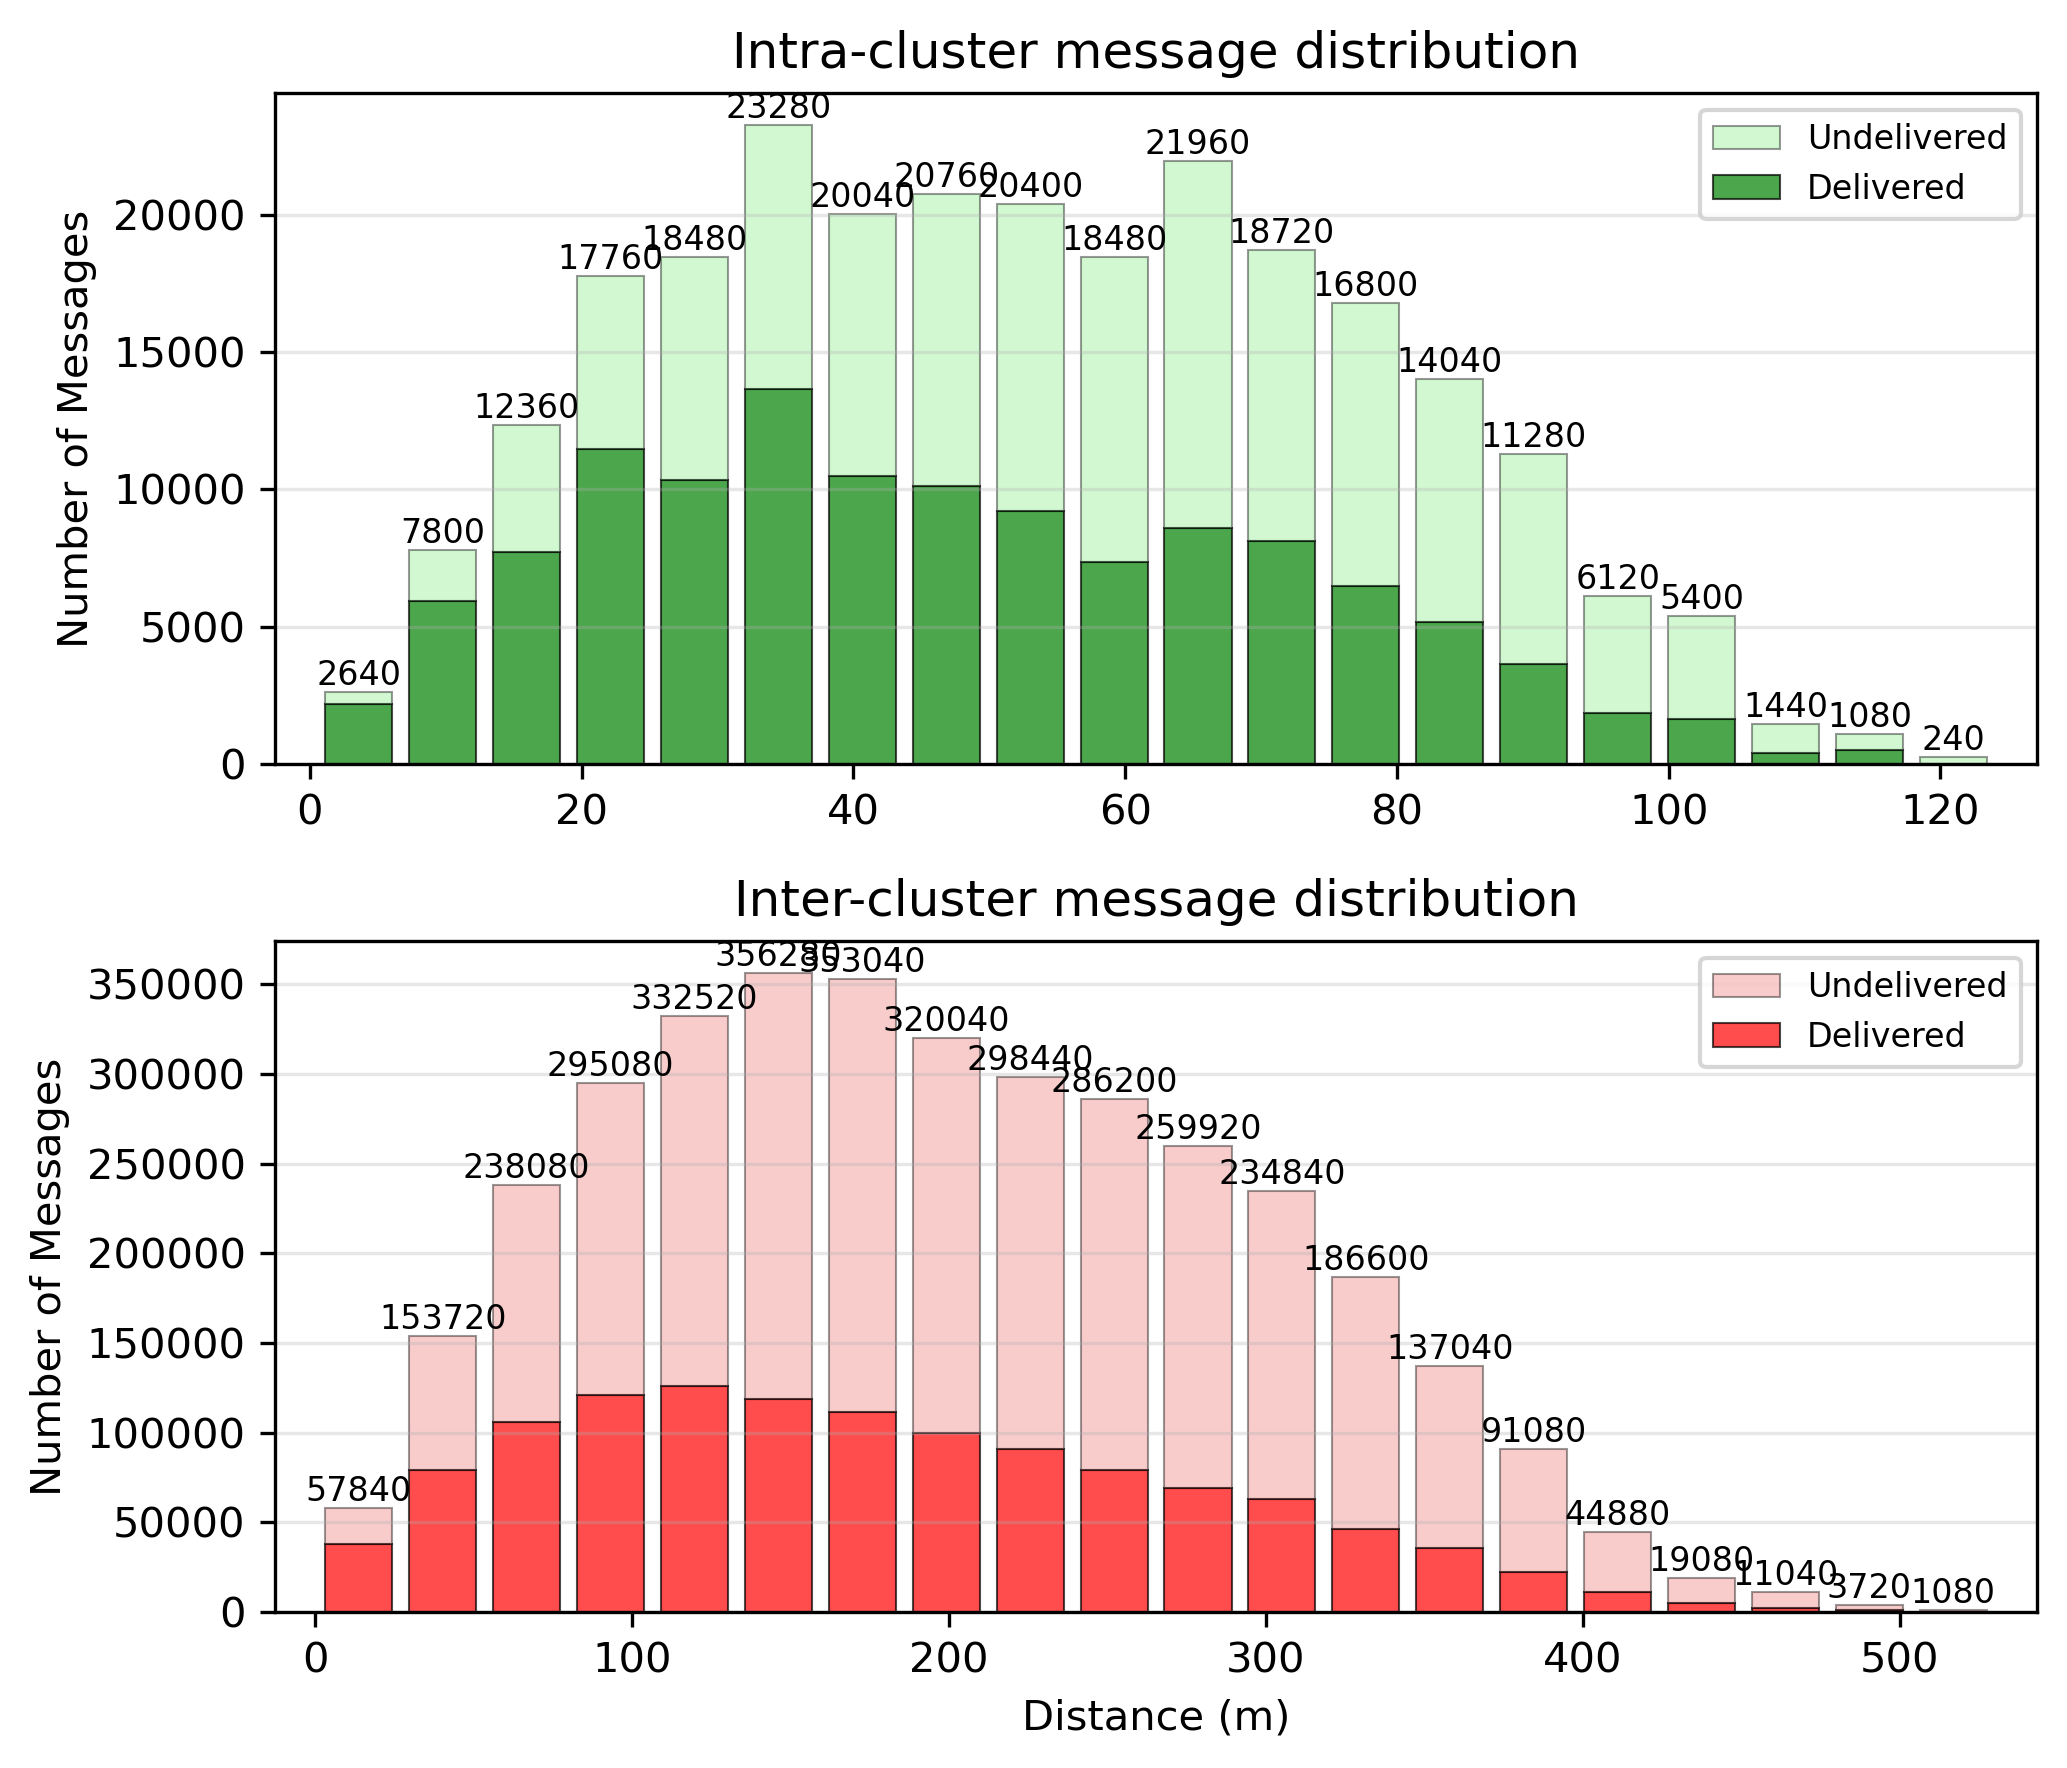
\includegraphics[width=0.5\textwidth]{figures/message_distance_distribution.png}
    \caption{Message Distance Distribution}
    \label{fig:message-distance-distribution}
\end{figure}

Figure \ref{fig:message-distance-distribution} shows the distance distribution of all messages created, aggregated over all simulation runs, communication ranges, and maximum node degrees tested, split by the communication mode. 
It is evident to see that the intra-cluster communication mode had a generally higher overall delivery probability, possibly attributed to a lesser strain on the individual hosts' message buffers.
\begin{figure}[hbp]
    \centering
    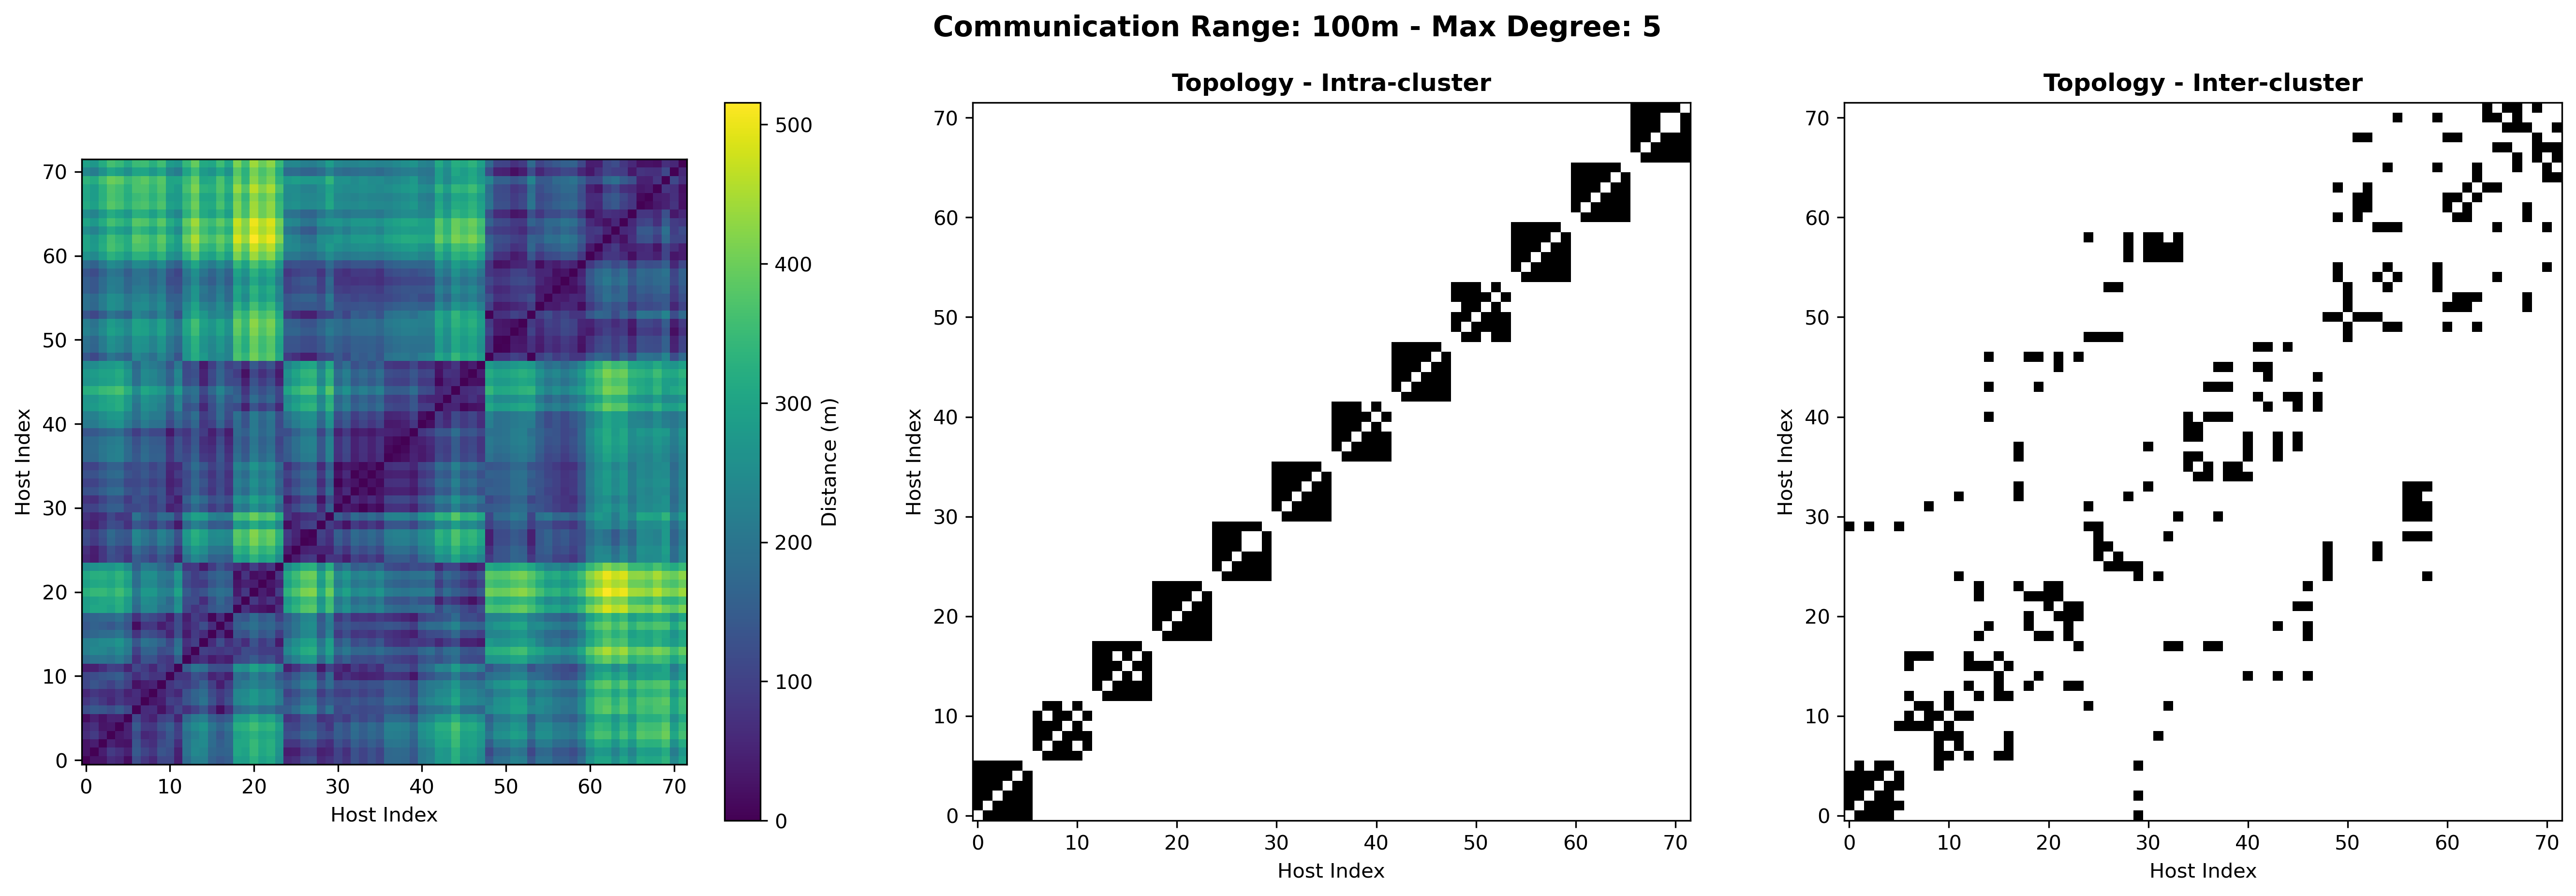
\includegraphics[width=0.5\textwidth]{figures/range100_maxdeg5_topology_distance.png}
    \caption{Topology and distance metrices for communication radius 100m, constrained maximum node degree 5}
    \label{fig:topology-matrix-100m-5}
\end{figure}
To better understand the topology, figure \ref{fig:topology-matrix-100m-5} shows the distance matrix between hosts to the left, supplemented by two topological matrices, one for each communication mode.
The topological matrices have a black cell at position $(i, j)$ if host $i$ is connected to host $j$.

Next, randomized topologies were created for each configuration, to assess how the maximum node degree affects the message latency, centralization, and sparsity metrics of unstructured p2p networks.
This was done to evaluate how different topologies with the same communication radius and maximum node degree induce variance in the different metrics 
% A configuration is composed of some properties: in this part, we chose to examine the affects of the per-node Bluetooth interface communication range parameter: as wireless signals exponentially degrade with distance, but the received signal strength correlates with the transmitted signal strength, we are interested in the trade-off between energy consumption and the deliverability of messages, as well as the achievable bitrate.
% For every simulation run, 1000 messages were generated for every distance bin: the following plot shows a summary of how the message creation distribution varies with range, collected from all runs. We can see a concentration around $\sim$25 meter distance, and a long tail that stretches all the way to $\sim$500 meter.
